\documentclass[12pt, a4paper, twopage]{scrartcl}


\usepackage{lmodern} 		% Diese beiden packages sorgen für echte 
\usepackage[T1]{fontenc}	% Umlaute.

\usepackage{amssymb, amsmath, color, graphicx, float, setspace, tipa}
\usepackage[utf8]{inputenc} 
\usepackage[ngerman]{babel}
\usepackage[pdfpagelabels,pdfstartview = FitH,bookmarksopen = true,bookmarksnumbered = true,linkcolor = black,plainpages = false,hypertexnames = false,citecolor = black, breaklinks]{hyperref}
\usepackage{url}
\usepackage{picins} 		%Gleittext um Grafik. Befehl: parpic. Vorlage siehe unten
\usepackage{longtable} 		%Seitenübergreifende Tabelle. Vorlage siehe unten
\usepackage{caption}
\captionsetup{font=small,labelfont=bf, format=plain, justification=centering}
\allowdisplaybreaks % allows page breaks in align/equation environment

%--------------------------------------------
% NEUE BEFEHLE
%--------------------------------------------
% Gleich mit Dach obendrauf
\newcommand{\entspricht}{\mathrel{\widehat{=}}}

% Atanh
\newcommand {\arctanh}{\mathrm{arctanh}}

% Acotanh
\newcommand{\arccot}{\mathrm{arccot }}

% Limes von etwas gegen null
\newcommand{\limz}[1]{\lim\limits_{#1 \rightarrow 0}}

%Bold font in math
\newcommand{\bm}{\boldmath}
\newcommand{\dps}{\displaystyle}

% e noncursive in math mode
\newcommand{\e}{\mbox{e}}

% partial diff operator
\newcommand{\del}{\partial}
%--------------------------------------------
%--------------------------------------------
%---------OPTIONAL---------------------------

%% Schriftart ändern
%\newcommand{\changefont}[3]{
%\fontfamily{#1} \fontseries{#2} \fontshape{#3} \selectfont}
%\changefont{ppl}{m}{n} nach \begin{document} einsetzen

%% Abb. statt Abbildung, Tab. statt Tabelle
%\usepackage[footnotesize]{caption2}
\addto\captionsngerman{\renewcommand{\figurename}{Abb.}}
%\renewcommand{\tablename}{Tab.}%

%\pagestyle{headings} % Überschrift an jeder Seite

%\usepackage{chngcntr} \counterwithout{figure}{section} % Ganzzahlige Bildnummerierungen, Kapitelunabhängig




%------------------------------------------------------------------
%------------------------------------------------------------------
%----------------VORLAGEN------------------------------------------
%----------------VORLAGEN------------------------------------------
%----------------VORLAGEN------------------------------------------
%------------------------------------------------------------------

%Bruch: \frac{}{}
%Kleiner Bruch: \tfrac{}{}
%Gleichungen: \begin{align}
%Delta für partielle Ableitungen: \partial
%Schönes Epsilon: \varepsilon

%Strich: in align-Umgebung, \bar{} oder \overline{}
%Seitenumbruch: \clearpage ; Besser als \newpage, da er floats zwingt, zuerst eingefügt zu werden.
%Zu grosse Zeilenabstände wegen Formelzeichen? -> \vphantom{}, \smash{}
%\newcommand{\BefehlName}[Anzahl_Parameter]{Definitiere neuen Befehl. Den ersten Parameter ruft man mit #1 ab, den zweiten mit #2 etc}

%%FIGUR
%\begin{figure}[htbp]
%\centering
%\includegraphics[width=15cm]{Bild1}%
%\caption{Experimental set-up}%
%\label{1}
%\end{figure}

%%BILD MIT PICINS NEBEN TEXT SETZEN
%\piccaption{Caption\label{label}} 
%\parpic[r]{\fbox{\includegraphics [width=5cm, keepaspectratio]{bild.png}}}
%


%% ZWEI BILDER NEBENEINANDER.
%% Schau, dass die minipages insgesamt nie mehr als 1.0\textwidth haben.
%% Um ein drittes oder viertes Bild einzufügen, ergänze einfach um weitere minipages.
% \begin{figure}[!htb]
% \centering
%   \minipage{0.3\textwidth}
%     \fbox{\includegraphics[height=2.5cm, keepaspectratio]{rsflipflop.png}}%
%     \caption{RS-Flipflop}%
%     \label{fig:rsflipflop}
%   \endminipage\hspace{1cm}   
% %
%   \minipage{0.4\textwidth}
%     \fbox{\includegraphics[height=2.5cm, keepaspectratio]{rsflipfloptakt.png}}%
%     \caption{getaktetes RS-Flipflop}%
%     \label{fig:rsflipfloptakt}
%   \endminipage
% \end{figure}



%% TABELLEN
%% 1) mit tabular
%\begin{center}
%\begin{tabular}[c]{|p{1cm}|p{3cm}|p{3cm}|p{3cm}|}
%\hline
%\multicolumn{2}{|c||}{Stromstärke 0.4A}	&	\multicolumn{2}{c|}{Stromstärke 0.6A}\\
%\hline
%$4T$ in s	&	$T'$		&	$4T$ in s	&	$T'$\\
%\hline
%7.1			&	1.775	&	7.1		& 	1.775\\
%\hline
%7.2			&	1.8		&	7.1		&	1.775\\
%\hline
%7.3			&	1.825	&	7.1		&	1.775\\
%\hline
%\end{tabular}
%\end{center}
%
%% 2) Mit longtable
%\begin{longtable}{p{3.5cm} p{11.5cm}}
%  Blabla & Blabla\\ [2mm] <= Macht 2mm Abstand zwischen Zeilen
%  %
%  Blabla & Blabla \\ [2mm]
%\end{longtable}


%%%%%%%%%%%%%%%%%%%%%%%%%%%%%%%%%%%%%%%%%%%%%%%%%%%%%%%%%%%%%%%%%%%%%%%%%%%%%%%%%%%%%%%%%%%%%%%%%%%%%%%%%%%%%%%%%%%%%%%%%%%%%%%%%%%%%%%%%%%%%%%%%%%%%%%%%%%%%%%%%%%%%%%%%%%%

%------------------------------------------
%:Metainformationen

\title{Titel}
\author{Mladen Ivkovic\\
mladen.ivkovic@uzh.ch\\
}
\date{Datum}

% \title[Kurzform]{Vortrag zur Berechenbarkeit}
%     Titel des Vortrages
% \subtitle[Kurzform]{Untertitel}
%     Untertitel
% \author[M. Schulz]{Michael Schulz}
%     Autor festlegen
% \institute[IfI -- HU Berlin]{Institut für Informatik\\ Humboldt-Universität zu Berlin}
%     Angabe des Institutes
% \date[26.05.06]{26. Mai 2006}
%     Datum der Präsentation, alternativ kann mittels \date{\today} auch das aktuelle Datum eingetragen werden.

%------------------------------------------


\begin{document}
%\pagestyle{plain}

\maketitle
\clearpage
\tableofcontents %Auf englisch wechseln: Ändere usepackage ngeman babel in english babel
\clearpage

\section*{Anmerkung des Autoren}

Dieser Abschnitt ist nicht nummeriert und nicht im Inhaltsverzeichnis. 


\begin{description}
  \item[Zweck] Dieses Dokument blablabla.
  \item[Punkt 2] Punkt 2
\end{description}

Sonstiger text: Bla blablabla blabla bla. Blabla bla. Blablablabal basdiga asdifsdjfh asdfjlsdfn uilsdfyjkzu shflsdf jhksdfui sf df,jhi afuil sdfuinm,j shsdfnm,,.
\clearpage


\section{Kapitel 1}
\subsection{Unterkapitel 1.1}
\subsubsection{Unterunterkapitel 1.1.1}

%
\piccaption{Darstellung des Zahlenbereichs des Zweierkomplements mit acht Stellen\label{fig:tabelle_zweierkomplement}}
\parpic[r]{%
  \fbox{
    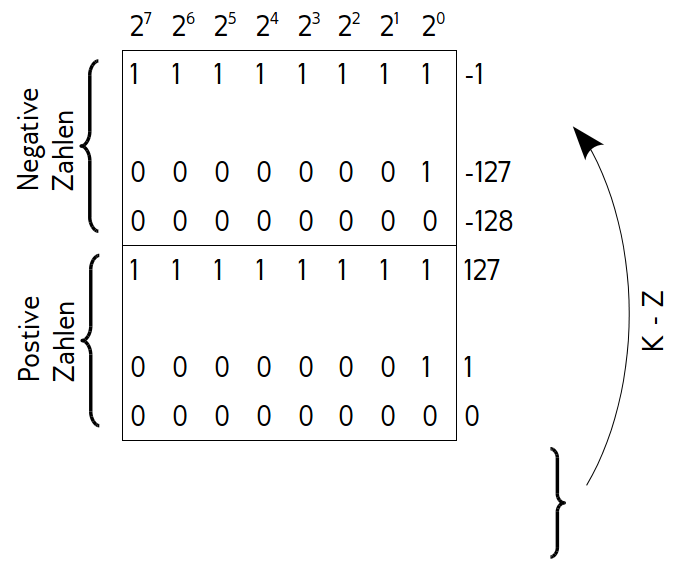
\includegraphics[width = 5.5cm, keepaspectratio]{Bilder/tabelle_zweierkomplement.png}
  }
}
%
Die gängigste Form der Zahlensysteme sind Stellenwertsysteme. Eine Zahl $a$ wird in Form einer Reihe von Ziffern $z_i$ mit dazugehöriger Potenz der Basis $b^i$ dargestellt. Der Wert der Zahl ergibt sich dann als Summe der Werte aller Einzelstellen: $a = \sum\limits_{i}z_ib^i$.

\textbf{Umrechnung} in andere Zahlensysteme: Gegeben sei Zahl $Z$, umzuwandeln in System mit Basis $b$.
Eine angenehme Vorgehensweise gibt uns das \textbf{Horner Schema}\footnote{
Website mit Umrechnungen und Erklärungen: \url{http://www.arndt-bruenner.de/mathe/scripts/Zahlensysteme.htm}
}: Dividiere $Z$ durch $b$. Der Rest dieser Division ist die letzte Stelle der Zahl in der Basis $b$  (Einerstelle). Dividiere den Quotienten dieser Division wieder durch $b$. Der Rest dieser zweiten Division ergibt die zweite Stelle der Zahl in der neuen Basis. Wiederhole Divisionen, bis kein Rest mehr.


\section{Tabellen}
\subsection{Einfach}
\begin{center}
\begin{tabular}[c]{c | c | c || c| c | c || c | c || c | c | c || c| c| c}
\multicolumn{3}{c||}{Konjunktion}	&	\multicolumn{3}{c||}{Disjunktion} & \multicolumn{2}{c||}{Negation} & \multicolumn{3}{c||}{NAND} & \multicolumn{3}{c}{NOR}\\
\multicolumn{3}{c||}{UND}	&	\multicolumn{3}{c||}{ODER} & \multicolumn{2}{c||}{} & \multicolumn{3}{c||}{} & \multicolumn{3}{c}{}\\
\hline
$a$ & $b$ & $a$ $\wedge$ $b$ & $a$ & $b$ & $a$ $\vee$ $b$ & $a$ & $\bar{a}$ & $a$ & $b$ & $\overline{a \wedge b}$ & $a$ & $b$ & $\overline{a \vee b}$\\
\hline
0 & 0 & 0 & 0 & 0 & 0 & 0 & 1 & 0 & 0 & 1 & 0 & 0 & 1\\
0 & 1 & 0 & 0 & 1 & 1 & 1 & 0 & 0 & 1 & 1 & 0 & 1 & 0\\
1 & 0 & 0 & 1 & 0 & 1 & & & 1 & 0 & 1 & 1 & 0 & 0\\
1 & 1 & 1 & 1 & 1 & 1 & & & 1 & 1 & 0 & 1 & 1 & 0\\
\hline
\end{tabular}
\end{center}

\subsection{Mit extra + Seitenumbruch}
\begin{spacing}{1.4}
\begin{longtable}{p{4cm} l l}
Kommutativgesetz: & $a \wedge b = b \wedge a$ & $a \vee b = b \vee a$\\ 
Distributivgesetz: & $a \wedge (b \vee c) = (a \wedge b) \vee (a \wedge b)$ & $a \vee (b \wedge c) = (a \vee b) \wedge (a \vee c)$\\ 
Neutrales Element & $a \wedge 1 = a$ & $a \vee 0 = a$\\
Inverses Element & $a \wedge \bar{a} = 0$ & $a \vee \bar{a} = 1$\\
Assoziativgesetz & $(a \wedge b) \wedge c = a \wedge (b \wedge c)$ & $(a \vee b) \vee c = a \vee (b \vee c)$\\
Idempotenzgesetz & $a \wedge a = a$ & $a \vee a = a$\\
Absorptionsgesetz & $a \wedge ( a \vee b) = a$ & $a \vee (a \wedge b) = a$\\
DeMorgan-Gesetz & $\overline{a\wedge b} = \bar{a} \vee \bar{b}$ (NAND)& $\overline{a \vee b} = \bar{a} \wedge \bar{b}$ (NOR)\\
\smash{Gesetz vom Widerspruch} & & $a \wedge \overline{a} = 0$\\
\smash{Gesetz vom ausgeschl. Dritten} & & $a \vee \overline{a} = 1$ \\
\smash{Gesetz der doppelten Negation} & & $\overline{\overline{a}} = a$ \\
\end{longtable}
\end{spacing}




%-----------------------------
\section{Zwei Bilder}

\begin{figure}[h!]
\centering
  \minipage{0.3\textwidth}
    \fbox{\includegraphics[height=2.5cm, keepaspectratio]{Bilder/rsflipflop.png}}%
    \caption{RS-Flipflop}%
    \label{fig:rsflipflop}
  \endminipage\hspace{1cm}   
%
  \minipage{0.4\textwidth}
    \fbox{\includegraphics[height=2.5cm, keepaspectratio]{Bilder/rsflipfloptakt.png}}%
    \caption{getaktetes RS-Flipflop}%
    \label{fig:rsflipfloptakt}
  \endminipage
\end{figure}

Dabei müssen wir eine Nebenbedingung $R \wedge S = 0$ setzen - $R$ und $S$ dürfen niemals gleichzeitig $= 1$ sein. In der Realisierung, dargestellt in Abb. \ref{fig:rsflipflop}, führt dies zu oszillationen. 

Will man ein taktgesteuertes RS-Flipflop, so braucht man lediglich das Taktsignal mit einem UND-Gatter jeweils mit dem $R$- und $S$-Eingang zu verbinden (siehe Abb. \ref{fig:rsflipfloptakt}).



\section{Mathematik und Symbole}



\begin{align}
	 & \equiv \ \ll \ \lll \ \gg \ \ggg \ \leq \ \geq \ \leqslant \ \geqslant \ \propto \ \approx \ \approxeq \ \neq \ \simeq \ \cong \ \ncong \\\
	 %
	 & \cdot \ \times \ \vee \ \wedge \ \veebar \ \barwedge \pm \ \mp \ \sqrt{a} \ \sqrt[3]{a} \ \langle \ \rangle \ \infty\\
	 %
	 & \leftarrow \ \rightarrow \ \Leftarrow \ \Rightarrow \ \parallel \ \bot \ \\
	 %
	 & \in \ \notin\ \forall \ \exists \ \nexists \ \ni \ \mathbb{RNZ} \ \subset \ \supset \ \subseteq \ \supseteq \ \\
	 %
	 & \int\limits_{1}^{2} \ \oint \ \iint \ \iiint \ \prod \ \sum \ \\
	 %
	 & \ \vec{r} \ \bar{r} \ \dot{r} \ \ddot{r} \ \mathbf{r} \ \underline{r} \\
	 %
	 & \odot \ \nabla \ \partial \ \hbar\\
	 %
	 %
	 %
	 %
	 \nonumber \\
	 %
	 \vec{S}_\mu &= \vec{S}_\mu ^{\parallel}(0) \vec{u} + \vec{S}_\mu^{\bot} (0) [\cos(\omega_\mu t)\vec{v} - \sin(\omega_\mu t)\vec{w}]\\
	 %
	 \vec{P} &= \frac{2}{\hbar} \langle \Psi | \hat{S} | \Psi \rangle = \vec{S}\\
	 %
	 %
	 % UNDERBRACE
	 \Rightarrow \varphi (x) &= \sum\limits_{L = 0}^{\infty} \sum\limits_{m = - L}^{L} \sqrt{\frac{4 \pi}{2 L + 1}}  \underbrace{\int\limits_{\mathbb{R}^3} \sqrt{\frac{4 \pi}{2 L + 1}} \rho(\vec{x} ' ) r'^{L} Y_{l, m}^{*} (\theta ', \varphi ') d^3 x'}_{q_{l,m}}  \frac{Y_{l,m}(\theta, \varphi)}{r^ {L + 1}} \\ 
	 %
	 &= \sum\limits_{L = 0}^{\infty} \sum\limits_{m = - L}^{L} \sqrt{\frac{4 \pi}{2 L + 1}} q_{l,m}  \frac{Y_{l,m}(\theta, \varphi)}{r^ {L + 1}}\\
	 % CASES
	 \nonumber
	 \Rightarrow q_{0, 0} &= \int \limits_{\mathbb{R}^3} \rho(\vec{x}' ) d^3 x' \entspricht 
	 \begin{cases} 
	 \text{total charge (electrostatics)} \\
	 \text{total mass (gravitation)}\\
	 \end{cases}\\
	 % 3dim-VECTOR
	 \vec{r} &= \left( \begin{matrix}
	 r \cos \varphi \sin \theta\\
	 r \sin \varphi \sin \theta\\
	 r \cos \varphi
	 \end{matrix} \right )\\
	 %
	 ... &=\begin{vmatrix}
		  -1-\lambda & 1 & -1 \\
		  2 & -1-\lambda & 2\\
		  2 & 2 & -1-\lambda\\
		  \end{vmatrix}\\
	 %
	 \begin{pmatrix}
	 0\\0\\0
	 \end{pmatrix} &= \begin{pmatrix}
	 0 & 1 & -1 \\
	 2 & 0 & 2\\
	 2 & 2 & 0\\
	 \end{pmatrix} \begin{pmatrix}
	 x_1 \\ y_1\\ z_1
	 \end{pmatrix}\\
	 %
	 z + \bar{z} &\leq 2\sqrt{z\bar{z}} \tag*{:2} \\\nonumber	 
	 %
	 Re(z) &\leq |z| = \sqrt{Re(z)^2 + Im(z)^2} \tag*{$\square$}\\
	 %
	 |\sin z| &\overset{3b)}= \sqrt{\sin^2 x}\\
	 %
	 \cosh(y) & \overset{y \in \mathbb{R}} \geq 1 \Rightarrow x = n \pi, n \in \mathbb{Z}\\
	 %
	 f(z) &= \lim\limits_{x\rightarrow \infty} \frac{\sin x}{x} = 0\\
	 %
	 f^{(n)} (z_0) &= \frac{n!}{2\pi i} \oint_C  \frac{f(z)}{(z - z_0)^{n + 1}}\\
	 %
	 \binom{a}{n} &= \frac{a!}{(a-n)! n!}\\
	 %
	 \nonumber \limz{\epsilon}\int(z) dz &= \limz{\epsilon} \frac14 \left[ \int\frac{e^{ia(u + 1)}}{u} du - \int\frac{e^{ia(u + 1)}}{u + 2}du   \right]\\[1em]
	 & \overset{z = 1 \Rightarrow u = 0}= \limz{\epsilon} \frac{e^{i a}}{4} \left[\vphantom{ \int\limits_{\pi}^0} \smash{ \underbrace{\frac{\overbrace{e^{ia \epsilon e^{i \varphi}}}^{\rightarrow 1}} {\epsilon e^{i \varphi}} i \epsilon e^{i \varphi}}_{\rightarrow i}  d \varphi            - \int\limits_{\pi}^0 \underbrace{\frac{\overbrace{e^{ia \epsilon e^{i \varphi}}}^{\rightarrow 1}} {\underbrace{\epsilon e^{i \varphi}}_{\rightarrow 0} + 2} \underbrace{i \epsilon e^{i \varphi}}_{\rightarrow 0}}_{\rightarrow 0}  d \varphi  }\right]\\[2em]
	 %	
	 %
	 2 + 2 &= 4 \ \text{some more space after this line please.}\\[4em]
	 %
	 \nonumber  2 + 2 &= 4 \text{ \hspace{1cm} unnumbered line.}\\
	 %
	 %
	 %
	 &\text{last line is made of text. Yay!}
\end{align}




In-line maths elements can be set with a different style: \(f(x) = \displaystyle \frac{1}{1+x}\). The same is true the other way around:

\begin{eqnarray*}
	f(x) = \sum_{i=0}^{n} \frac{a_i}{1+x} \\
	\textstyle f(x) = \textstyle \sum_{i=0}^{n} \frac{a_i}{1+x} \\
	\scriptstyle f(x) = \scriptstyle \sum_{i=0}^{n} \frac{a_i}{1+x} \\
	\scriptscriptstyle f(x) = \scriptscriptstyle \sum_{i=0}^{n} \frac{a_i}{1+x}
\end{eqnarray*}
















%##########################################################################3
%##########################################################################
%3#########3###############################################################
\clearpage
\begin{appendix}
\setcounter{figure}{0} %Bildnummerierung auf Null setzen
\renewcommand{\thefigure}{A\arabic{figure}} %Bilder mit A$Bildnummer beschriften
\section{Bildanhang}


\begin{figure}[h!]
\centering
\minipage{0.4\textwidth}
  \fbox{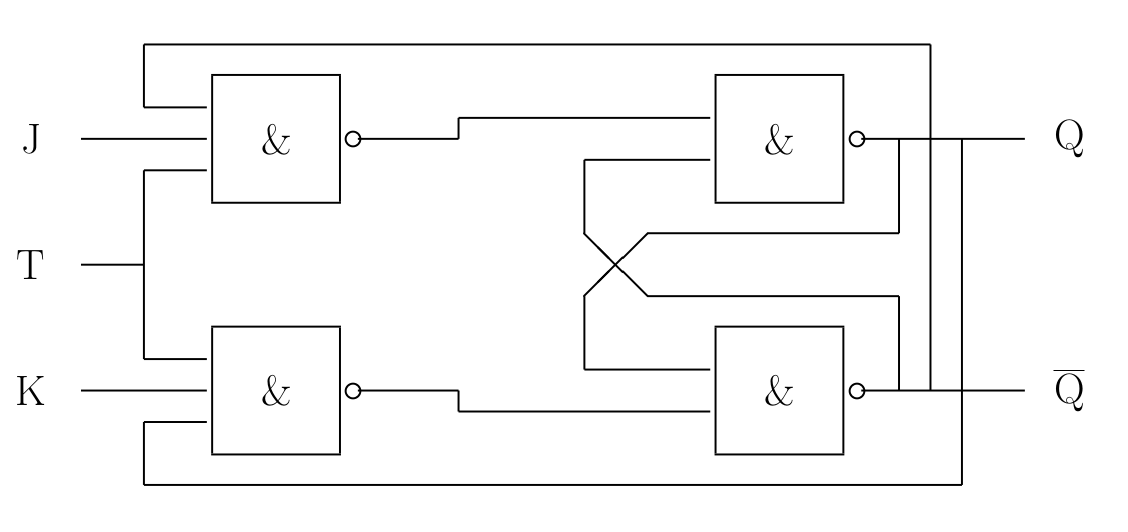
\includegraphics[height = 3cm, keepaspectratio]{Bilder/jkflipflop.png}}%
  \caption{JK-Flipflop \vspace{27pt}}%
  \label{fig:jkflipflop}
\endminipage\hspace{.5cm}
%
\minipage{0.4\textwidth}
  \fbox{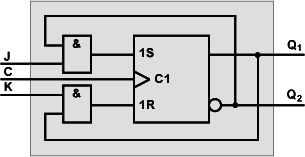
\includegraphics[height = 3cm, keepaspectratio]{Bilder/JKmitRS.png}}%
  \caption{JK-Flipflop, Darstellung mit RS-Flipflop. C = Takt, $Q_1 = Q$, $Q_2 = \bar{Q}$}%
  \label{fig:JKmitRS}
\endminipage
\end{figure}

\section{Zeilenumbruch}
asdfghjklösdfghjklösdfghjklöasdfghjklösdfghjklösdfghj111klöasdfghjklösdfghjklösdfghjklöasd222\-fghjklösdfghjklösdfghjklöasdfghjklösdfghjklösdfghjklöasdfghjklösdfghjklö


\section{Neue Befehle definieren}
\newcommand{\musr}{$\mu$SR }
\musr


\newcommand{\myint}{\int\limits_{-\infty}^{\infty} dr \int\limits_{0}^{2 \pi} \sin(\vartheta) \varepsilon d\varphi}

\newcommand{\mysum}[3]{\sum\limits_{j = 0}^{\infty} \frac{#1\cdot #2}{#3} e^{- 3 \cos(\theta \phi)}}

\begin{align*}
  &\text{myint} & \myint\\
  &\text{mysum} & \mysum{x}{y}{z}
\end{align*}

\renewcommand{\myint}{myint ist jetzt ein neuer Befehl und macht nur noch das hier.}

\myint

\vspace{2cm}
\newcommand{\fett}[1]{{\bf #1}}

\fett{fettes hallo}

\newcommand{\kursiv}[1]{{\it #1}}

\kursiv{kursives hallo}



\end{appendix}
\end{document}